\documentclass[12pt,a4paper,notitlepage]{article}

\usepackage[utf8]{inputenc}

\usepackage[francais]{babel}\usepackage[T1]{fontenc}
\usepackage[cyr]{aeguill}
\usepackage{lmodern}
\usepackage{listings}
\lstset{language=bash, basicstyle=\footnotesize, frame=shadowbox, rulesepcolor=\color{gris}}

\usepackage{amssymb}
\usepackage[table]{xcolor}
\definecolor{gris}{gray}{0.75}
\definecolor{bleup}{HTML}{258EE9}


%\renewcommand*\familydefault{\ttdefault} %% Only if the base font of the document is to be typewriter style
%\renewcommand{\rmdefault}{ptm}


\usepackage[
   pdfauthor={Ludovic Terrier & Arnaud Goulut},
   pdftitle={RE12 - TP1},
   ]{hyperref}
   
   
\usepackage[pdftex]{graphicx}

%\usepackage{titlesec}
%\titleformat{\section}[frame] {\normalfont} {\filright
%\footnotesize
%\enspace\textbf{\thesection}\enspace} {8pt} {\Large\bfseries\filcenter}

%% Je contrôle la taille de ma zone imprimée...
\usepackage{anysize}
%% ...en définissants les marges {gauche}{droite}{haute}{basse}
\marginsize{25mm}{15mm}{10mm}{15mm}

\begin{document}

\title{La configuration réseau sous Linux}
\author{Ludovic Terrier et Arnaud Goulut}
\date{Mars 2010}
\maketitle


%\tableofcontents

\thispagestyle{empty}
\newpage

%%%%%%%%%%%%%%%%%%%%%%%%%%%%%%%%%%%  1ère page 


%%%%%%%%%%%%%%%%%%%%%%%%%%%%%%%%%%% 1ère partie
\section{Partie 1}

\subsection{Plan de câblage du réseau}
\begin{figure}[!h]
\begin{center}
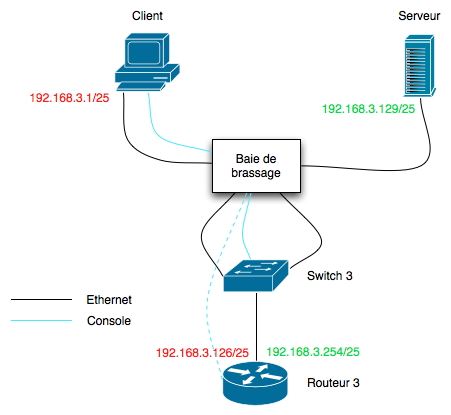
\includegraphics[height=11cm]{Diag.png}
\caption{Présentation du réseau configuré au cours du TP.}
\label{fig:do}
\end{center}
\end{figure}

\subsection{Configuration IP}
\paragraph{}Dans les réseaux du serveur et du client on utilise un seul réseau (192.168.3.0) de classe C. Cependant pour en faire deux réseaux distincts on le scinde à l'aide du masque : $\mathtt{/25}$. Ceci signifie que les 25 premiers bits de chaque adresse IP utilisée sur le réseau correspondra au NetID et les 7 derniers au HostID. On obtient donc 2 sous-réseaux ayant pour adresse respective : 192.168.3.0 et 192.168.3.128.

\paragraph{}Dans le cas du réseau de transport, nous avons un réseau 172.16.3.0, qui contiendra seulement deux machines. C'est pourquoi on peut se permettre d'utiliser un masque $\mathtt{/30}$ qui, appliqué à notre réseau de départ, donne 4 adresses : 
\begin{itemize}
\item deux adresses à utiliser pour des hosts,
\item une pour le broadcast,
\item une pour le NetID.\\
\end{itemize}

Ci-dessous les configurations des 3 réseaux :
\begin{center}
\rowcolors{1}{gris}{}
\begin{tabular}{| c | c | }
  \hline
 \multicolumn{2}{|c|}{\cellcolor{bleup}\textcolor{white}{Réseau du client}} \\
  \hline
  NetID & 192.168.3.0 \\
  Masque & /25  \\
  Plage d'adresse & 192.168.3.0 - 192.168.3.127\\
  1\up{ère} adresse machine & 192.168.3.1\\
  Dernière adresse machine & 192.168.2.126\\
  Nombre de machines potentiel & 126\\
  Broadcast & 192.168.3.127\\
  \hline
\end{tabular}
\end{center}

\begin{center}
\rowcolors{1}{gris}{}
\begin{tabular}{|c|c|}
  \hline
  \multicolumn{2}{|c|}{\cellcolor{bleup}\textcolor{white}{Réseau du seveur (DMZ)}} \\
  \hline
  NetID & 192.168.3.128 \\
  Masque & /25  \\
  Plage d'adresse & 192.168.3.128 - 192.168.3.255\\
  1\up{ère} adresse machine & 192.168.3.129\\
  Dernière adresse machine& 192.168.3.254\\
  Nombre de machines potentiel & 126\\
  Broadcast & 192.168.3.255\\
  \hline
\end{tabular}
\end{center}

\begin{center}
\rowcolors{1}{gris}{}
\begin{tabular}{|c|c|}
  \hline
  \multicolumn{2}{|c|}{\cellcolor{bleup}\textcolor{white}{Réseau de transport}} \\
  \hline
  NetID & 172.16.3.0 \\
  Masque & /30  \\
  Plage d'adresse & 172.16.3.0 - 172.16.3.3\\
  1\up{ère} adresse machine & 172.16.3.1\\
  Dernière adresse machine&  172.16.3.2\\
  Nombre de machines potentiel & 2\\
  Broadcast & 172.16.3.3\\
  \hline
\end{tabular}
\end{center}




\subsection{Configuration des équipements via le port console}

Pour l'administration de matériel réseaux on préfère utiliser un port console dédié. Ceci afin d'assurer l'accès à l'équipement en cas de mauvaise manipulation, qui le rendrait inaccessible via ses interfaces réseaux (Ethernet dans le cadre des TPs) ou dans le cas d'une congestion du réseau. On s'affranchit alors de tout problème d'adressage.\\

Cette interface a un port série (avec connectique RJ45 et DB9) 


\section{Partie 2}
\subsection{Configuration du switch}

Deux sous-réseaux sont connectés au switch, c'est pourquoi nous devons le séparer logiquement. Ceci est effectué grâce aux Virtual Local Area Networks (VLANs). Une différenciation des deux VLANs peut se faire par ports, ce qui se voit dans le fichier de configuration des switchs, seul le port \textit{FastEthernet0/2} est attribué à un VLAN :

\begin{center}
\fbox{
	\begin{minipage}{8cm}
	\hspace{2cm}\vdots\\
	{\small interface FastEthernet0/2}\\                        
	{\small switchport access vlan 2} 
	 
	 
	 \hspace{2cm}\vdots
	 \end{minipage}
}
 \end{center}
 
Ce qui peut vouloir dire que l'ensemble des autres ports sont dans le même VLAN par défaut.

\subsection{Configuration du routeur}
\paragraph{}Le switch de notre réseau étant relié au routeur par un seul médium et que celui-ci transporte les flux de deux sous-réseaux, il faut que l'interface routeur soit elle-même séparée en deux interfaces logiques. Ce qui semble fait au regard du fichier de configuration du routeur :


\begin{center}
\fbox{
	\begin{minipage}{8cm}
	\hspace{2cm}\vdots\\
	{\small interface FastEthernet0/0\textbf{.1}}\\                           
	 {\small encapsulation dot1Q 1 native}\\                             
	 {\small ip address 192.168.3.126 255.255.255.128}\\                                         
	{\small ! }\\
	{\small interface FastEthernet0/0\textbf{.2}}          \\                 
	 {\small encapsulation dot1Q 2}               \\
	 {\small ip address 192.168.3.254 255.255.255.128}  
	 
	 
	 \hspace{2cm}\vdots
	 \end{minipage}
}
 \end{center}



L'interface \textit{FastEthernet0/0} du routeur à laquelle est connectée le switch est partagée en deux : 
\begin{itemize}
\item \textbf{.1} pour le réseau 192.168.3.0 (l'interface ayant l'adresse 192.168.3.126)
\item \textbf{.2 }pour le réseau 192.168.3.128 (l'interface ayant l'adresse 192.168.3.254)
\end{itemize}


\section{Partie 3}
\subsection{/etc/sysconfig/network}
Pour communiquer sur un réseau, une machine nécessite une passerelle par défaut, mais peut aussi avoir besoin d'un nom. Ce sont donc ces informations que l'on s'autorise à stocker dans le fichier $\mathtt{/etc/sysconfig/network}$

\begin{center}
\fbox{
	\begin{minipage}{12cm}
	{\small HOSTNAME= azerty}\\
	{\small GATEWAY=192.168.1.254}
	 \end{minipage}
}
 \end{center}

\subsection{Pilote de la carte réseau}
\paragraph{}En lisant le fichier $\mathtt{/etc/modprobe.conf}$ on peut lire la ligne :

\begin{center}
\fbox{
	\begin{minipage}{8cm}
	\hspace{2cm}\vdots\\
	{\small alias eth1 e1000e}
	 
	 
	 \hspace{2cm}\vdots
	 \end{minipage}
}
 \end{center}

Ce qui signifie que l'alias \textit{eth1} est créé vers le pilote (\textit{e1000e}) de la carte réseau. Si l'on effectue la commande \textit{ifconfig} dans un Terminal on pourra observer \textit{eth1} et pas \textit{e1000e}.

\subsection{Paramètres de l'interface réseau}

Les paramètres que l'on peut attribuer à une interface réseau avec la commande \textit{ifconfig} sont l'adresse IP et le masque de sous réseau. Ceci est effectué grâce à la commande suivante :\\

\begin{lstlisting}
ifconfig <interface> <adresse_IP> netmask <masque>
\end{lstlisting}

Pour le Client :
\begin{lstlisting}
ifconfig eth1 192.168.3.1 netmask 255.255.255.128
\end{lstlisting}

Pour le Serveur :
\begin{lstlisting}
ifconfig eth1 192.168.3.129 netmask 255.255.255.128 
\end{lstlisting}
\vspace{0.3cm}


On peut aussi, à l'aide de cette commande, activer ou désactiver l'interface :

\begin{lstlisting}
ifconfig eth1 up
\end{lstlisting}

\begin{lstlisting}
ifconfig eth1 down
\end{lstlisting}
 
\subsection{Pérenniser les paramètres de l'interface réseau}

Les informations concernant l'adresse IP et le masque peuvent-être conservées de manière pérenne dans le fichier : $\mathtt{/etc/sysconfig/network-scripts/ifcfg-\textless interface\textgreater}$ 
ou dans notre cas $\mathtt{/etc/sysconfig/network-scripts/ifcfg-eth1}$\\

Il suffit de l'éditer et d'y ajouter :

\begin{center}
\fbox{
	\begin{minipage}{12cm}
	{\small IPADDR=\textless adresse\_IP\textgreater}\\
	{\small NETMASK=\textless masque\textgreater}
	 \end{minipage}
}
 \end{center}

Pour le poste Client :

\begin{center}
\fbox{
	\begin{minipage}{12cm}
	{\small IPADDR=192.168.0.1}\\
	{\small NETMASK=255.255.255.0}
	 \end{minipage}
}
 \end{center}

\subsection{Table de routage}
La table de routage donne à une machine le premier saut qui lui permet d'atteindre n'importe quelle autre machine située n'importe où sur l'Internet. \\

\begin{lstlisting}
route add -net <reseau_destination> netmask <masque> <interface>
\end{lstlisting}
Où  \textless interface\textgreater\ est l'interface à utiliser pour atteindre la destination.\\

De plus, cette table contient une route par défaut qui est utilisée par la machine en dernier recours. On parle alors de \textit{passerelle} ou de \textit{gateway}. Pour la signifier à une machine on tape la commande : \\

\begin{lstlisting}
route add default gw <adresse_IP_passerelle>
\end{lstlisting}
\vspace{0.8cm}
Exemple d'une table de routage affichée par la commande : \textit{route}.
{\footnotesize \begin{verbatim}
[root@server][~] route                                                                                                                                  
Kernel IP routing table
Destination     Gateway         Genmask         Flags Metric Ref    Use Iface
192.168.1.0  		  *               255.255.255.128 U     0      0        0 eth0
default         192.168.1.126   0.0.0.0         UG    0      0        0 eth0

\end{verbatim}}

Considérons la machine 192.168.1.23 avec la table ci-dessus, désirant communiquer avec 192.168.1.34. La machine va donc lire sa table de routage, s'apercevoir que la destination appartient au même sous-réseau qu'elle (grâce au masque) et va pouvoir lui remettre directement (\og \textbf{*} \fg).\\

Si la destination, par exemple un serveur de mails avec l'IP 93.56.134.23, n'est pas sur le même sous-réseau qu'elle, la machine va parcourir toute la table jusqu'à la fin. A la ligne \textit{default} elle va trouver l'adresse de la passerelle qui sera censée transférer les paquets jusqu'à la destination.

\subsection{Question 6}
Le DNS (Domain Name System) permet de faire la correspondance entre une adresse IP et un nom d'hôte. Ainsi, une personne désirant accéder à un site internet saisira dans son navigateur \url{www.utt.fr} au lieu de 193.50.230.241. Ce qui est beaucoup plus facile à retenir.\\

Les correspondances insérées dans le fichier $\mathtt{/etc/hosts}$ sont consultées en premier par le système, ce qui peut donc poser des problèmes de sécurité si ces dernières redirigent de manière transparente l'utilisateur vers un site non désiré.\\

\noindent La ligne correspondant à la manière dont le système va résoudre les noms dans le fichier $\mathtt{nsswitch.conf}$ est :


\begin{center}
\fbox{
	\begin{minipage}{8cm}
	\hspace{2cm}\vdots\\
	{\small hosts:    files dns}
	 
	 
	 \hspace{2cm}\vdots
	 \end{minipage}
}
 \end{center}


\emph{files} correspond au fichier $\mathtt{/etc/hosts}$ et \emph{dns} désigne l'utilisation du resolveur. Ainsi, le système d'exploitation consultera dans un premier temps le fichier puis s'il n'a pas trouvé de correspondance, il utilisera le service DNS via son resolveur.\\

Mais le fichier $\mathtt{nsswitch.conf}$ comporte également les réglages pour d'autres bases de données telles que :

\begin{center}
\fbox{
	\begin{minipage}{8cm}
	\hspace{2cm}\vdots\\
	{\small
passwd:     files ldap
	
shadow:     files ldap

group:      files ldap}
	 
	 
	 \hspace{2cm}\vdots
	 \end{minipage}
}
 \end{center}



\noindent \emph{passwd} définit l'endroit où le système doit chercher les utilisateurs (ici en local et sur un annuaire), \emph{shadow} est son équivalent mais pour les utilisateurs dont les mots de passe sont chiffrés. Enfin \emph{group} désigne les emplacements où sont répertoriés les groupes auxquels les utilisateurs appartienent.


\subsection{Outils de l'administrateur}
Il existe de nombreux outils pour l'administrateur réseau, en voici quelques uns.
\subsubsection{dig}

Dig permet de tester la résolution DNS via un autre serveur que celui configuré sur l'hôte, mais également de consulter l'ensemble des enregistrements d'un nom de domaine. Ce qui est utile pour diagnostiquer un dysfonctionnement dans la résolution des noms.\\

Avec la commande ci-dessous, on effectue une recherche inversée permettant de retrouver la machine qui porte cette IP.

{\footnotesize \begin{verbatim}
[root@server][~] dig -x 193.50.230.240 +short
pluton.utt.fr.
\end{verbatim}}

\subsubsection{host}

La commande host permet d'effectuer des requêtes DNS de manière simplifiée. On peut consulter les enregistrements pour un domaine précisé et ainsi vérifier le bon fonctionnement de son service DNS. Dans l'exemple suivant, la commande host nous indique l'ensemble des IPs enregistrées sous le nom de domaine \emph{smtp-in.orange.fr}.


{\footnotesize \begin{verbatim}
[root@server][~]  host  smtp-in.orange.fr
...
smtp-in.orange.fr has address 193.252.22.65
smtp-in.orange.fr has address 80.12.242.15
smtp-in.orange.fr has address 80.12.242.142
smtp-in.orange.fr has address 193.252.22.92
...
\end{verbatim}}

\subsubsection{nmap}
C'est un outil très complet, permettant de faire des analyses du réseaux pour retrouver les hôtes présents, les ports ouverts sur une machine, mais également de la détection de systèmes d'exploitations. Il permet donc de détecter l'ensemble des machines sur le réseaux ainsi que leurs failles potentielles.\\

\noindent Dans la capture suivante, on voit pour l'adresse IP scannée qu'il y a six ports ouverts, ainsi que leurs services associés.

{\footnotesize \begin{verbatim}
[root@server][~] nmap 188.165.75.22
Host is up (0.063s latency).
Not shown: 992 filtered ports
PORT      STATE  SERVICE
22/tcp    open   ssh
25/tcp    open   smtp
80/tcp    open   http
110/tcp   open   pop3
143/tcp   open   imap
443/tcp   open   https
8080/tcp  closed http-proxy
10000/tcp closed snet-sensor-mgmt
\end{verbatim}}

\subsubsection{traceroute}

Traceroute permet de suivre le chemin qu'un paquet IP va prendre pour aller d'une machine A vers une machine B. Ce qui est utile pour vérifier que nos paquets prennent bien le chemin escompté. \\

Dans l'exemple suivant, on voit l'ensemble des machines par lesquelles un paquet IP est passé pour contacter google.fr.

{\footnotesize \begin{verbatim}
[root@server][~] traceroute google.fr
traceroute to google.fr (209.85.229.104), 30 hops max, 40 byte packets
 1  ks305635.kimsufi.com (91.121.221.12)  0.000 ms  0.000 ms  0.000 ms
 2  rbx-63-m1.routers.ovh.net (91.121.221.253)  4.000 ms  0.000 ms  0.000 ms
 3  91.121.130.1 (91.121.130.1)  12.000 ms * *
 4  20g.ldn-1-6k.routers.chtix.eu (91.121.131.14)  4.000 ms * *
 5  195.66.224.125 (195.66.224.125)  4.000 ms  4.000 ms  4.000 ms
 6  64.233.175.27 (64.233.175.27)  8.000 ms  4.000 ms  8.000 ms
 7  72.14.232.134 (72.14.232.134)  8.000 ms  8.000 ms  8.000 ms
 8  ww-in-f104.1e100.net (209.85.229.104)  12.000 ms  12.000 ms  12.000 ms
\end{verbatim}}

\subsubsection{netstat}

La commande netstat permet d'afficher des statistiques sur les connexions réseaux, les ports en écoute et les sessions TCP établies.\\

Dans l'exemple ci-dessous, netstat permet de lister l'ensemble des ports en écoute sur le serveur, permettant ainsi de savoir quel service est en fonctionnement.
{\footnotesize \begin{verbatim}
[root@server][~] netstat -atulpe
Connexions Internet actives (serveurs et établies)
Proto    Adresse locale          Adresse distante        Etat        User    
tcp      *:ldap                  *:*                     LISTEN      root                
tcp      *:sunrpc                *:*                     LISTEN      root       
tcp      *:munin                 *:*                     LISTEN      root     
tcp      *:ftp                   *:*                     LISTEN      proftpd   
tcp      *:ssh                   *:*                     LISTEN      root        
tcp      *:3128                  *:*                     LISTEN      root         
\end{verbatim}}

%\clearpage
\subsubsection{ping}
Ping est un outil simple mais très pratique. Il permet de vérifier si l'on peut contacter une machine, de connaître le temps moyen pour effectuer le parcours, mais aussi des statistiques telles que le nombres de paquets perdus, le nombre de routeurs traversés (via le ttl), \ldots

{\footnotesize \begin{verbatim}
[root@server][~] ping www.yahoo.fr                                                     
PING rc.fy.b.yahoo.com (206.190.60.37) 56(84) bytes of data.
64 bytes from w2.rc.vip.re4.yahoo.com (206.190.60.37): icmp_seq=1 ttl=56 time=88.0 ms
64 bytes from w2.rc.vip.re4.yahoo.com (206.190.60.37): icmp_seq=2 ttl=56 time=88.0 ms
^C
--- rc.fy.b.yahoo.com ping statistics ---
2 packets transmitted, 2 received, 0\% packet loss, time 1004ms
rtt min/avg/max/mdev = 88.000/88.000/88.000/0.000 ms      
\end{verbatim}}


\end{document}
